\documentclass[../main]{subfiles}

\begin{document}
\begin{frame}[standout]

We interpret the world in constrained ways

\visible<2>{It's how we cope with too much information}

\end{frame}

\begin{frame}{scientific forestry}
  \begin{columns}
  \begin{column}{0.6\textwidth}
  \centering
\includegraphics<1>[width=\textwidth]{../figures/zoom/1.png}
\includegraphics<2>[width=\textwidth]{../figures/zoom/2.png}
\includegraphics<3>[width=\textwidth]{../figures/zoom/3.png}
\includegraphics<4>[width=\textwidth]{../figures/zoom/4.png}
\includegraphics<5-6>[width=\textwidth]{../figures/zoom/5.png}
\includegraphics<7>[width=\textwidth]{../figures/high_modernist_city.png}

\end{column}
  \begin{column}{0.4\textwidth}
  \centering
  \visible<6>{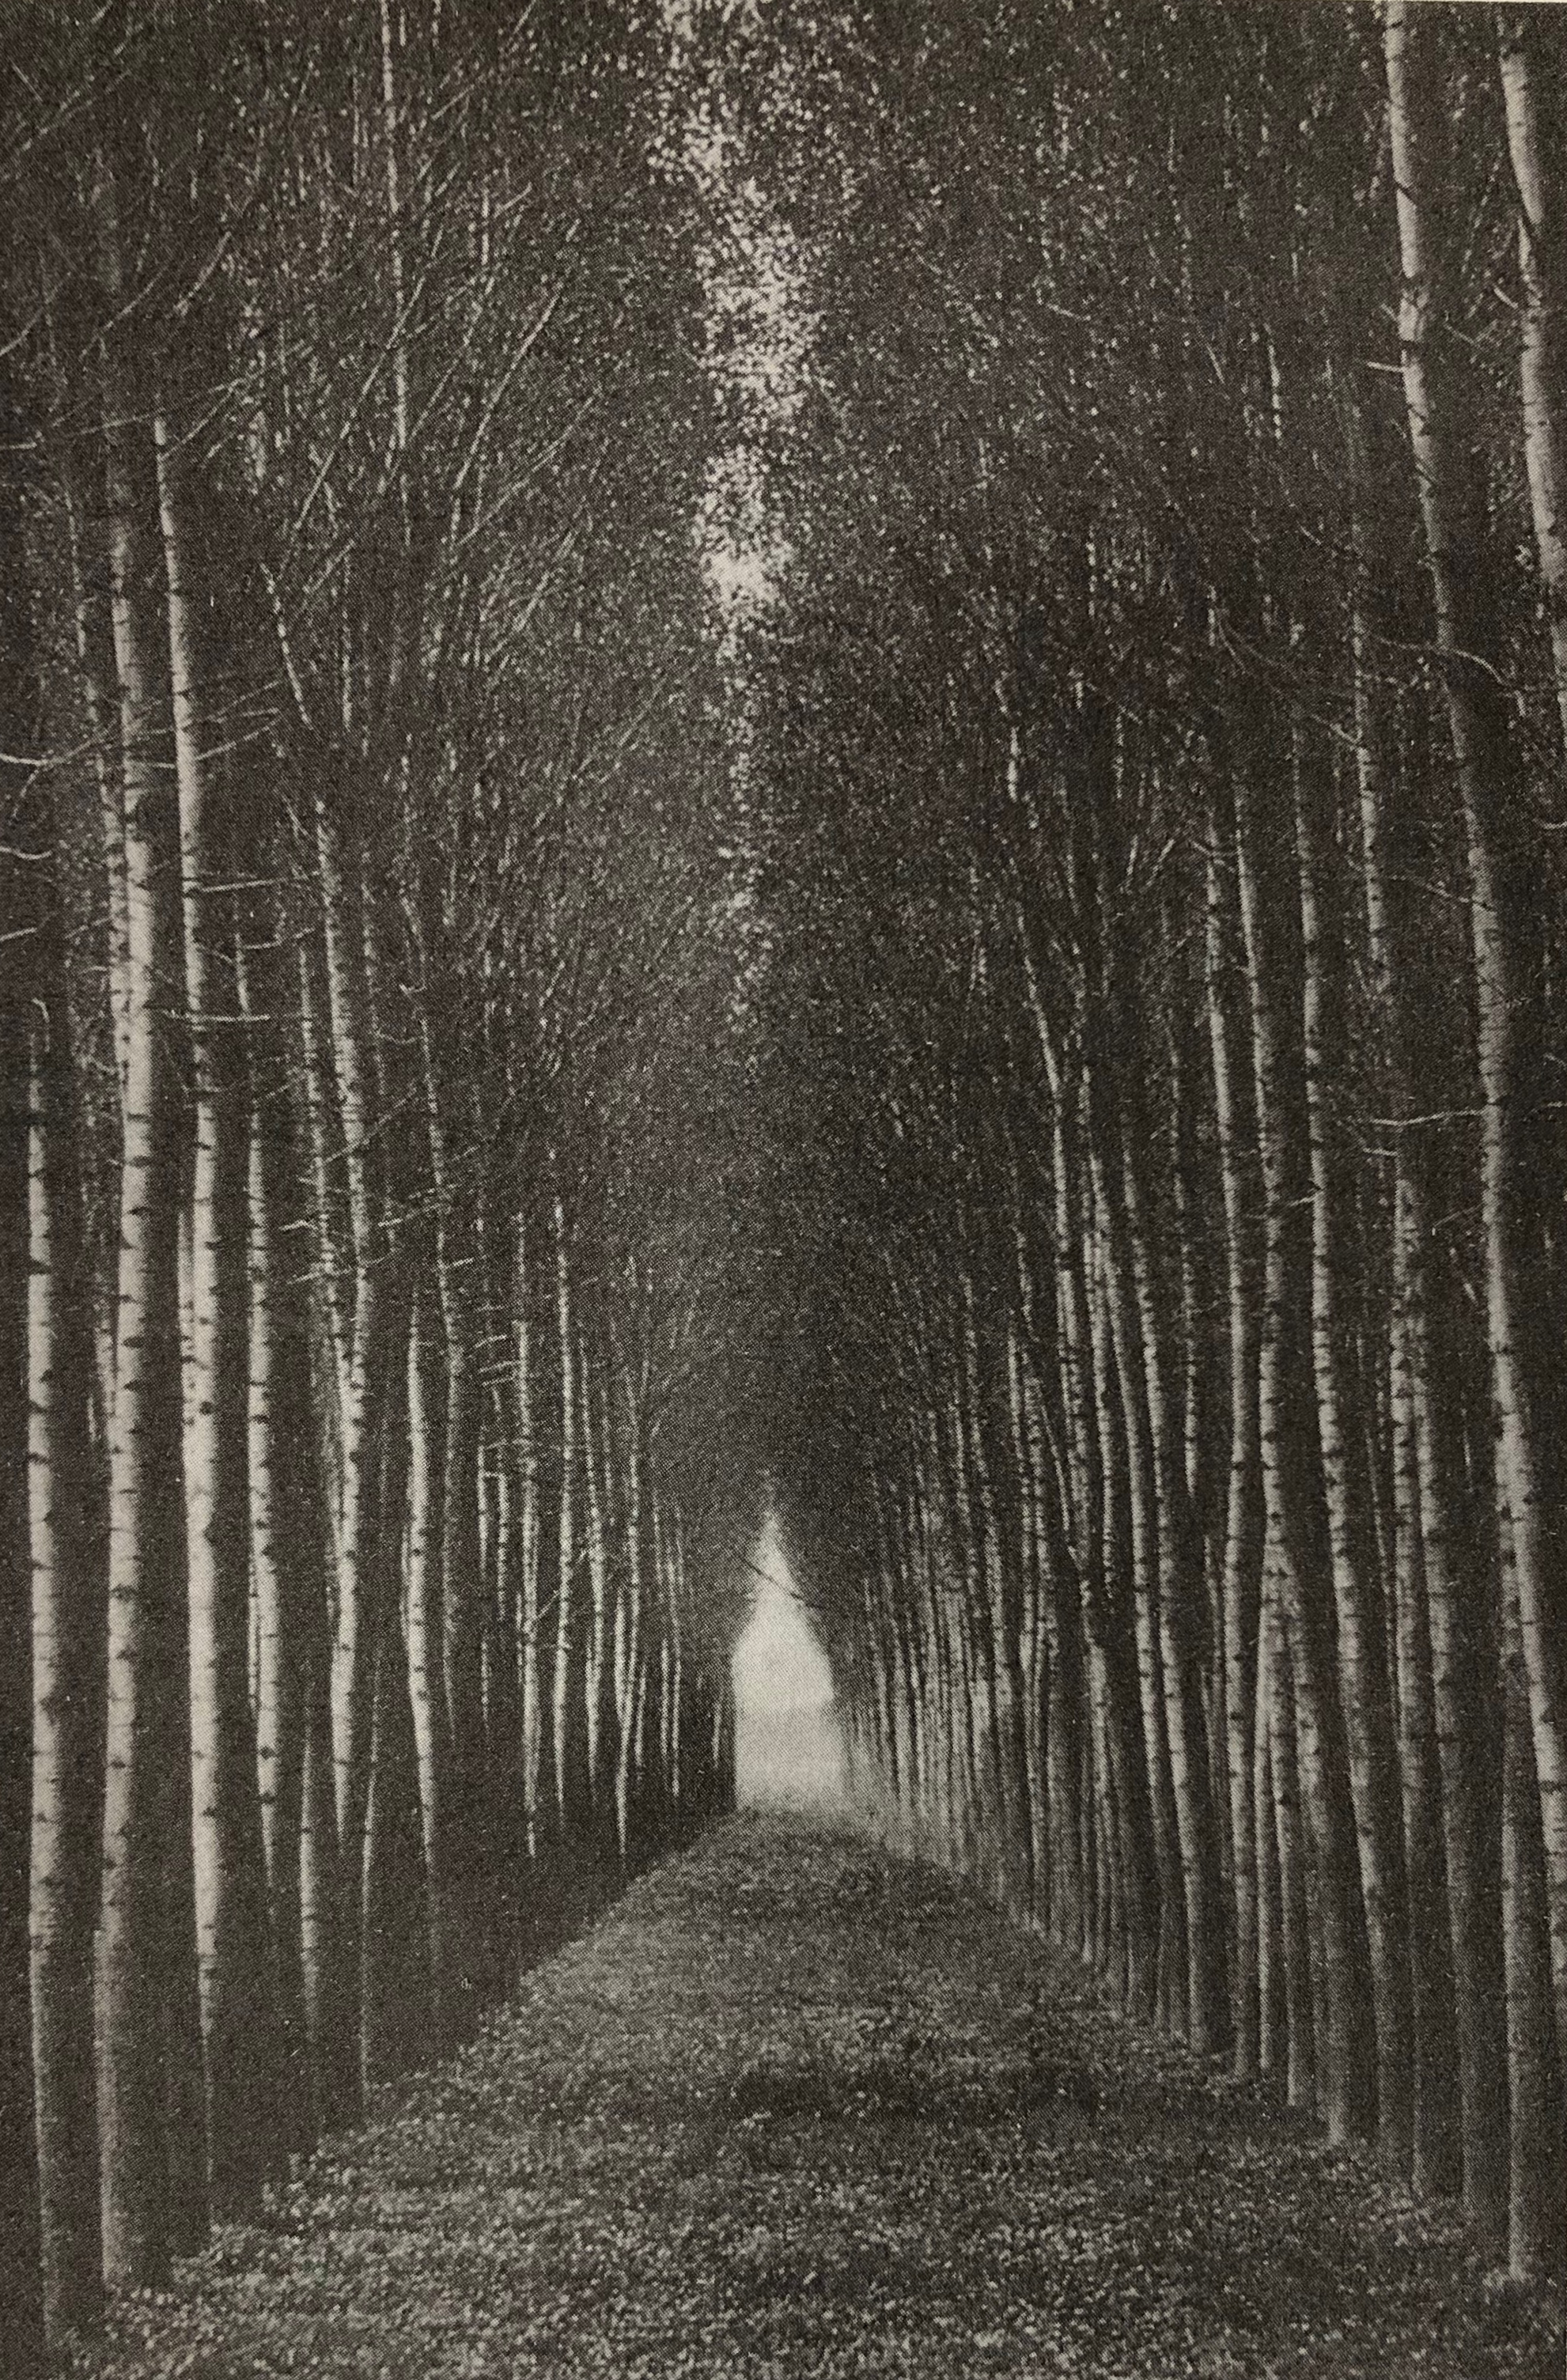
\includegraphics[height=0.8\textheight]{../figures/scifor.jpg}}

  \end{column}
  \end{columns}

\end{frame}


\begin{frame}[t]{delayed disasters}
  \begin{itemize}
    \visible<+->{\item Things were fine for a while}
    \visible<+->{\item Then they weren't}
      \visible<+->{\begin{itemize}
              \visible<+->{
                \item<+->[] Pests
                \item<+->[] Storms
                \item<+->[] Hollowing out of the ecosystem
              }
            \end{itemize}}
  \end{itemize}

\vfill

\centering
\visible<+->{\textit{\LARGE Waldsterben}

\visible<+->{\textit{\large{Forest death}}}
}

\vfill

\end{frame}


\begin{frame}{ecological diversity}

  \visible<+->{\alert{The forest} was more than just the trees}

  \visible<+->{It was everything that lived in and passed through}

\end{frame}


\end{document}